\chapter{Experimento I: Medición directa de la velocidad de la luz}
 
 A continuación se explica el primer experimento realizado, el cual busca medir directamente la velocidad de la luz. Se expone el funcionamiento, el método experimental, el análisis de los datos y los resultados obtenidos; así mismo, se enumeran algunas mejoras realizadas en búsqueda de una mayor precisión. Por último, se calcula la precisión necesaria con este experimento para poder verificar la \ac{HCC} en las localidades planteadas, lo cual explica por qué no es factible el experimento.
 

\section{Introducción}
Para verificar la \ac{HCC} la opción más evidente es la de medir directamente la velocidad de la luz en localidades con diferente densidad de energía, usando los mismos equipos y el mismo método cada vez. Un método sencillo para esto consiste en usar el haz de un láser modulado, el cual se divide haciendo que uno recorra una distancia mucho mayor y variable, y el otro una distancia corta y constante, ambos haces llegan a un mismo sensor donde se estudia el desfase entre ambas señales. El desfase $\Delta t$ aumenta si se aumenta la diferencia de camino $\Delta x$, ya que la relación entre ambos es

\begin{equation} \label{pendiente_c}
    \Delta x = c \Delta t
\end{equation}

de modo que al variar $\Delta x$ se puede trazar una recta cuya pendiente es la velocidad $c$.


\section{Método experimental}

\subsection{Materiales}

\begin{itemize}
    \item Láser de He-Ne
    \item Lente
    \item Espejo con soporte y tornillos de ajuste
    \item Divisor de haz
    \item Generdor de señales moduladas con fotodetectores
    \item Osciloscopio Tektronix TDS 2024B 
\end{itemize}

\subsection{Procedimiento experimental}
Para el montaje experimental se han usado dos variantes. La primera es la usada en la práctica de “Determinación de la velocidad de la luz” en Laboratorio 3 de la \ac{USB} \cite{GUIAlab3}, el esquema se puede ver en la figura \ref{fig:experimento_guia}.


\begin{figure}[hbt]
\centering
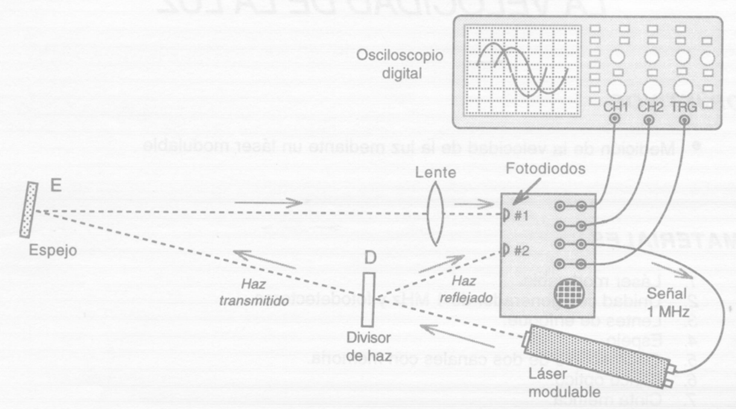
\includegraphics[scale=0.75]{experimento_guia.png}
\caption[]{Esquema experimental para la medición de la velocidad de la luz \cite{GUIAlab3}.}
\label{fig:experimento_guia}
\end{figure}


Se requiere de un láser de He-Ne conectado a un equipo generador de señales moduladas que además tiene incorporados dos fotodetectores, y un osciloscopio en cuyos dos canales se conectaron las señales recibidas por los detectores. La luz del láser pasa por un divisor de haz, el haz reflejado llega a uno de los detectores y el haz transmitido viaja hasta reflejarse en un espejo, y finalmente pasa por un lente que lo enfoca en el otro detector. El espejo se colocó en el extremo opuesto del salón, cada medida tomada se corresponde con una distancia diferente del espejo. Las distancias medidas, usando una cinta métrica convencional, se hicieron directamente de la diferencia de camino entre ambos haces. Para la segunda variante del montaje se reemplazó la señal proveniente del divisor de haz con la misma señal modulada que entra en el láser, mediante una conexión coaxial tipo T, el resto permaneció igual. 

\section{Análisis de datos}
Se usaron dos formas de medir el desfase, una directamente en la pantalla del osciloscopio usando los cursores y mediciones del mismo, y la otra forma extrayendo los datos digitales y haciendo el respectivo análisis. Para las medidas realizadas en la pantalla con los cursores del osciloscopio se ajustaron las dos señales hasta superponerse con amplitudes parecidas y se midió el desfase temporal entre ambas varias veces, tratando de medir siempre la misma parte de la curva. Esta manera de hacerlo permite calcular un promedio que será más fiel al desfase real.

Para la segunda forma, se debe tomar en cuenta que los datos que arroja el osciloscopio utilizado, Tektronix TDS 2024B, vienen en una carpeta de varios archivos, dos .csv cada uno con los valores de las ondas de luz recibidas, una foto de la pantalla del osciloscopio y un archivo .set que no se usó. Para el análisis de los datos (tiempo y voltaje) contenidos en las tablas de los archivos csv es necesario hacer un ajuste sinusoidal de la curva, esto con el fin de identificar las fases de cada una de las señales y poder calcular el desfase entre ellas. 

\begin{figure}[hbt]
\centering
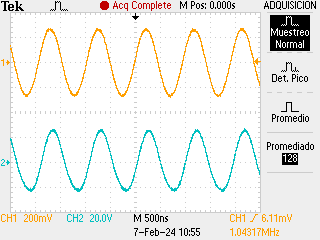
\includegraphics[scale=0.65]{F0003TEK.png}
\caption[]{Ejemplo de imagen de la pantalla del osciloscopio Tektronix TDS 2024B.}
\label{fig:osciloscopio}
\end{figure}

Para hacer el ajuste sinusoidal se creó un programa sencillo con el lenguaje Python. El funcionamiento del programa se basa en 4 etapas, la primera de ellas extrae los datos de tiempo y voltaje del csv. La segunda calcula los parámetros iniciales de búsqueda para el posterior ajuste, donde la frecuencia se calcula usando la Transformada Rápida de Fourier (FFT) de los datos e identificando la frecuencia de mayor amplitud; y la amplitud de la curva usando el cálculo de la desviación estándar. En la tercera etapa se usa la función \textit{curve\_fit}, que al pasarle los parámetros iniciales calculados antes los optimiza para minimizar la diferencia entre los datos de entrada y los valores calculados por la función sinusoidal, a través de métodos de mínimos cuadrados no lineales. Por último, en la cuarta etapa se grafica la curva original junto con la ajustada y se devuelven los parámetros de ajuste. La función de ajuste usada es la siguiente:

\begin{equation}
    A Sin(t \cdot \omega + \phi) + offset
\end{equation}
Por lo que el $\phi$ que arroja el programa está en radianes y debemos transformarlo a tiempo, esto se logra usando
\begin{equation}
    \Delta t = 2 \cdot \frac{|\phi_2 - \phi_1 | }{\omega_2 - \omega_1}
\end{equation}
Donde los subíndices se refieren a cada señal, note que la frecuencia angular usada en esta expresión es un promedio de las dos frecuencias encontradas.


Ya que se aclaró cómo encontrar el desface $\Delta t$ para ambos tipos de medidas realizadas, ahora es necesario calcular la velocidad de la luz. Para ello se usó Excel, donde se grafica $\Delta x$ vs $\Delta t$, recordando que $\Delta x$ es la medida realizada en el laboratorio. Finalmente, usando la formula de pendiente \ref{pendiente_c} se calcula la velocidad de la luz para cada conjunto de medidas. 

\begin{figure}[hbt]
\centering
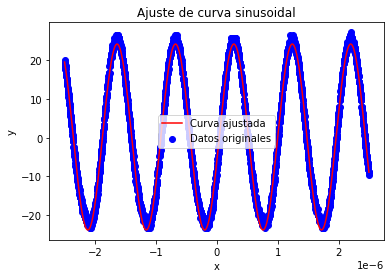
\includegraphics[scale=0.60]{AjusteF0003CH2.png}
\caption[]{Ejemplo de la imagen que devuelve el programa que hace el ajuste de la curva sinusoidal.}
\label{fig:ajusteLaser}
\end{figure}

\section{Resultados}

En cuatro diferentes oportunidades se hicieron mediciones de entre 4 y 7 distancias distintas para probar el montaje, con diferencias de camino entre 10 metros y los 30 metros. Se encontraron resultados poco precisos que se pueden observar en las figuras \ref{fig:C_resultados_malos}, donde todas las gráficas deberían ser una línea recta, y en la tabla \ref{tab:C_resultados_malos} donde se incluyen las pendientes calculadas.


\begin{table}[h]
\centering
\begin{tabular}{|l|l|l|}
\hline
n &  Pendiente (m/s$^2$) \\
\hline
1 & $(3.1666\pm 9.4493)\times 10^8$ \\

2 & $(0.2838\pm0.5678)\times10^8$  \\

3 & $(-0.2135\pm0.2775)\times10^8$\\
4.1 & No aplica \\
4.2 & No aplica \\
\hline
\end{tabular}
\caption{Valores de pendiente y su error para cada medida realizada.}
\label{tab:C_resultados_malos}
\end{table}





\begin{figure}[h!]
    % Primera fila
    \begin{subfigure}[b]{0.5\linewidth}
        \centering
        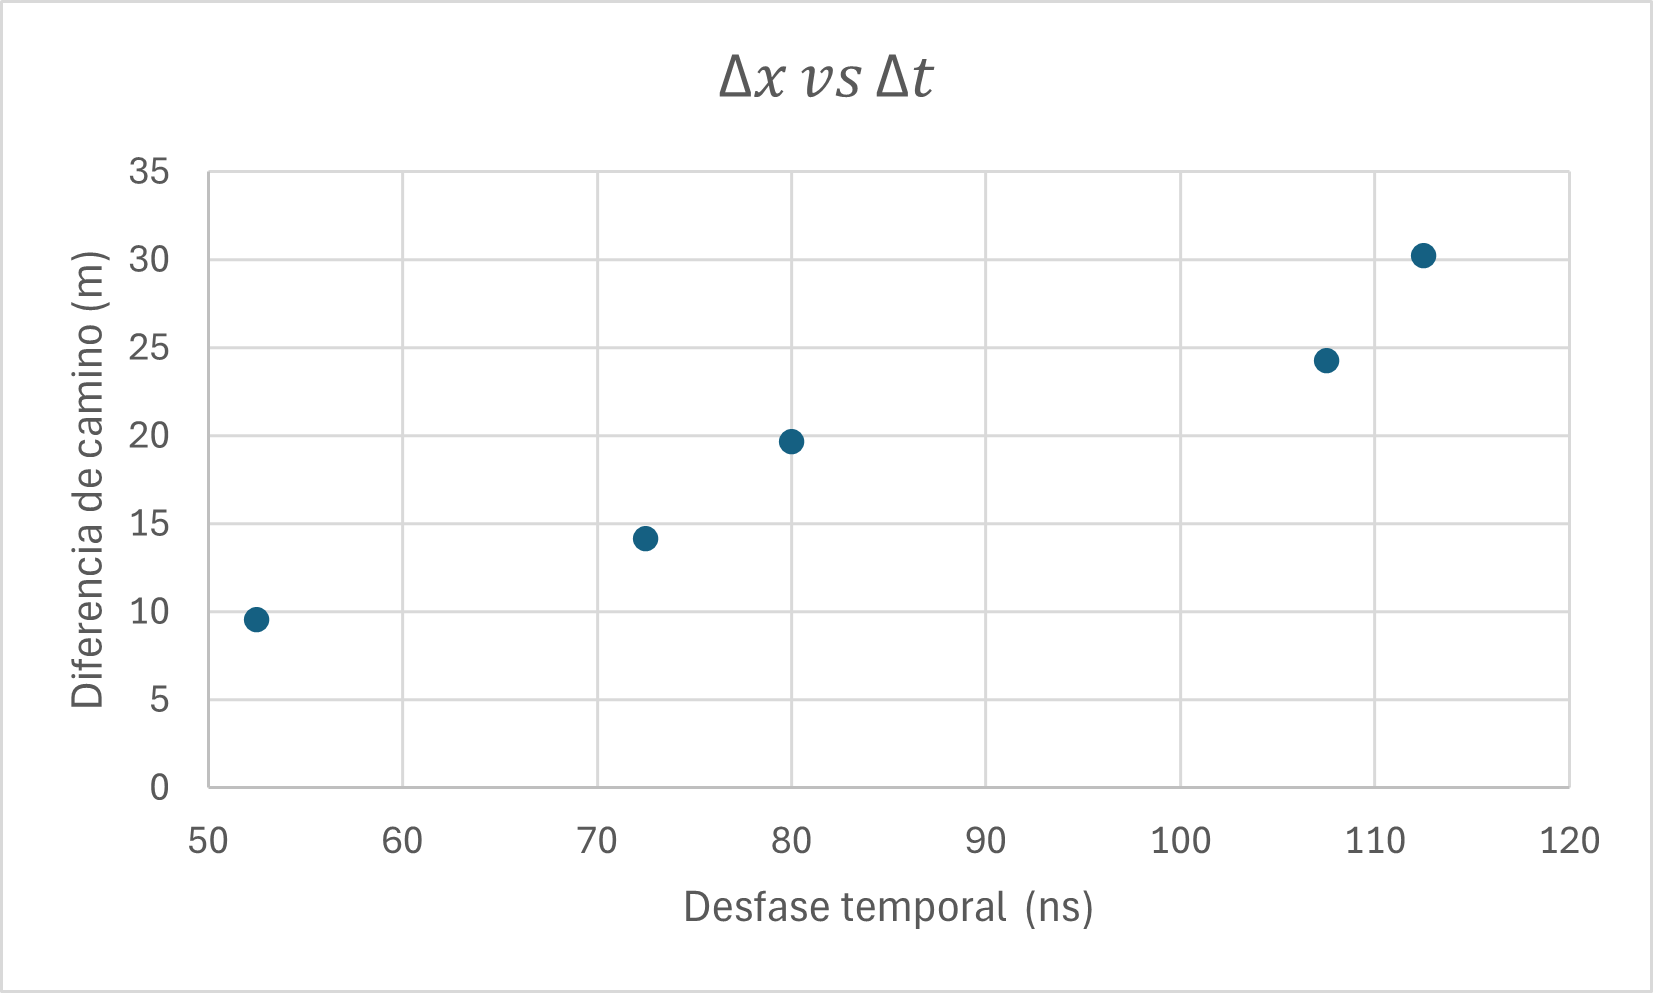
\includegraphics[width=\linewidth]{n-1.png} 
        \caption{Medida n1}
        \label{fig:n1}
    \end{subfigure}
    \hfill
    \begin{subfigure}[b]{0.5\linewidth}
        \centering
        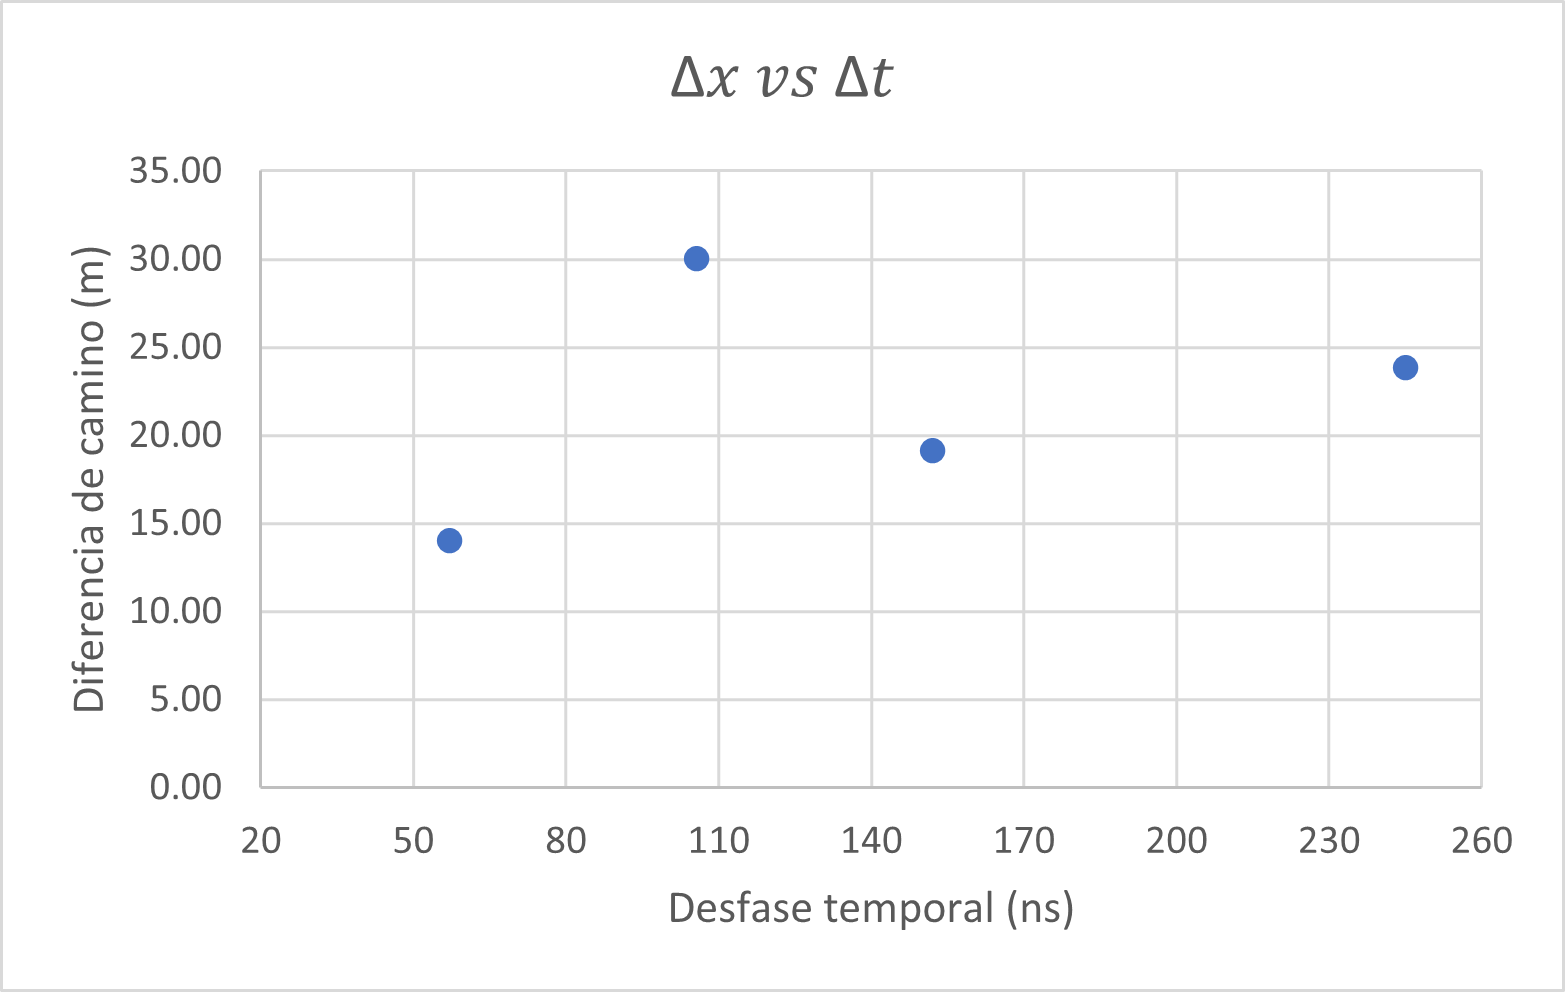
\includegraphics[width=\linewidth]{n-2.png} % Ruta de la segunda imagen
        \caption{Medida n2}
        \label{fig:n2}
    \end{subfigure}

    % Segunda fila
    \vspace{1em}
    \begin{subfigure}[b]{0.5\linewidth}
        \centering
        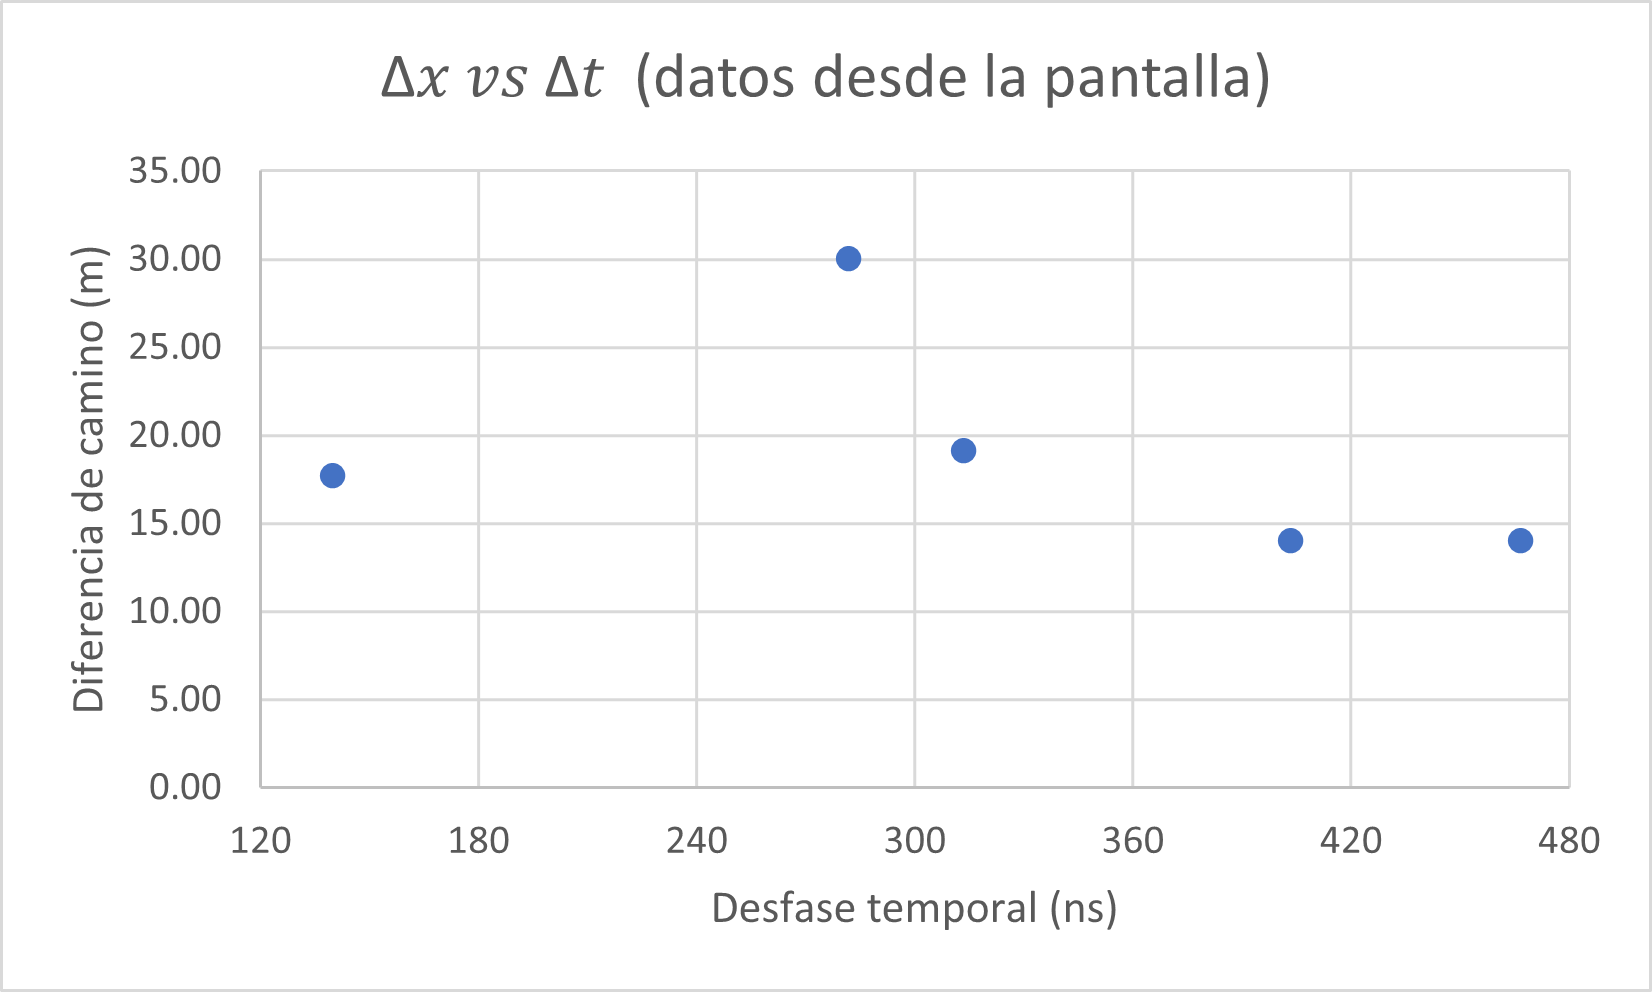
\includegraphics[width=\linewidth]{n-3.png} % Ruta de la tercera imagen
        \caption{Medida n3}
        \label{fig:n3}
    \end{subfigure}
    \hfill
    \begin{subfigure}[b]{0.5\linewidth}
        \centering
        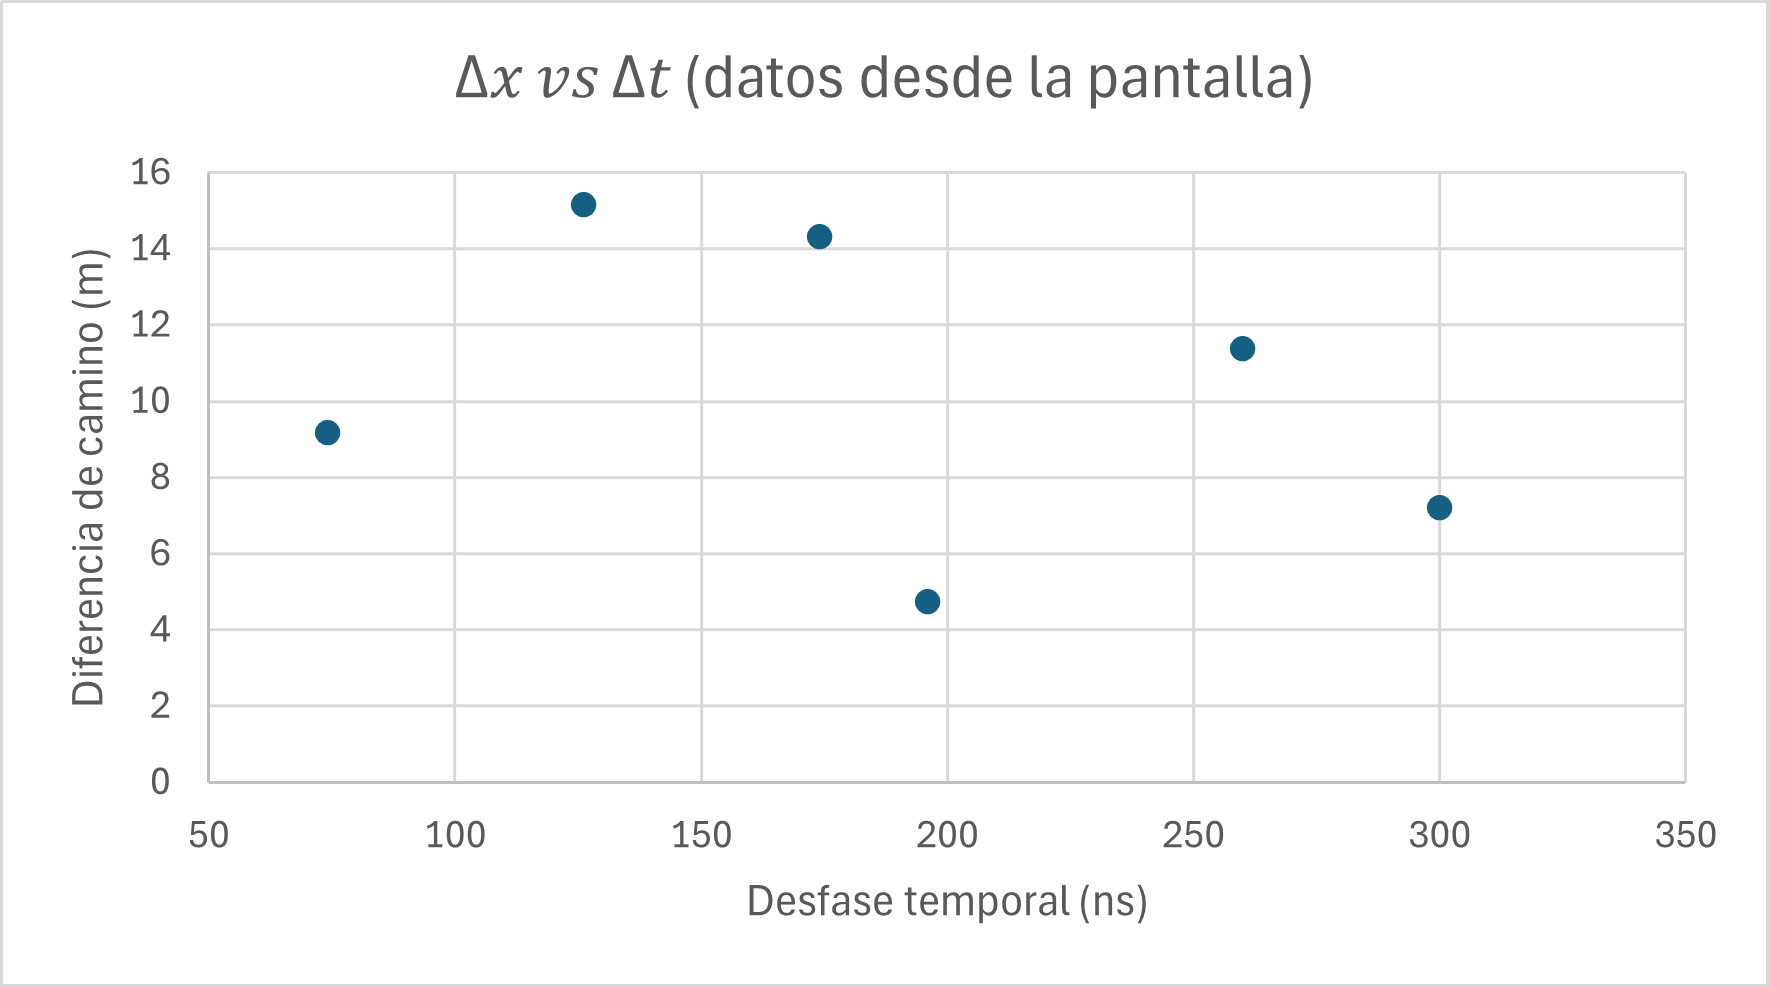
\includegraphics[width=\linewidth]{n-4.1.png} % Ruta de la cuarta imagen
        \caption{Medida n4.1}
        \label{fig:n4.1}
    \end{subfigure}

    % Tercera fila
    \vspace{1em}
    \begin{subfigure}[b]{0.5\linewidth}
        \centering
        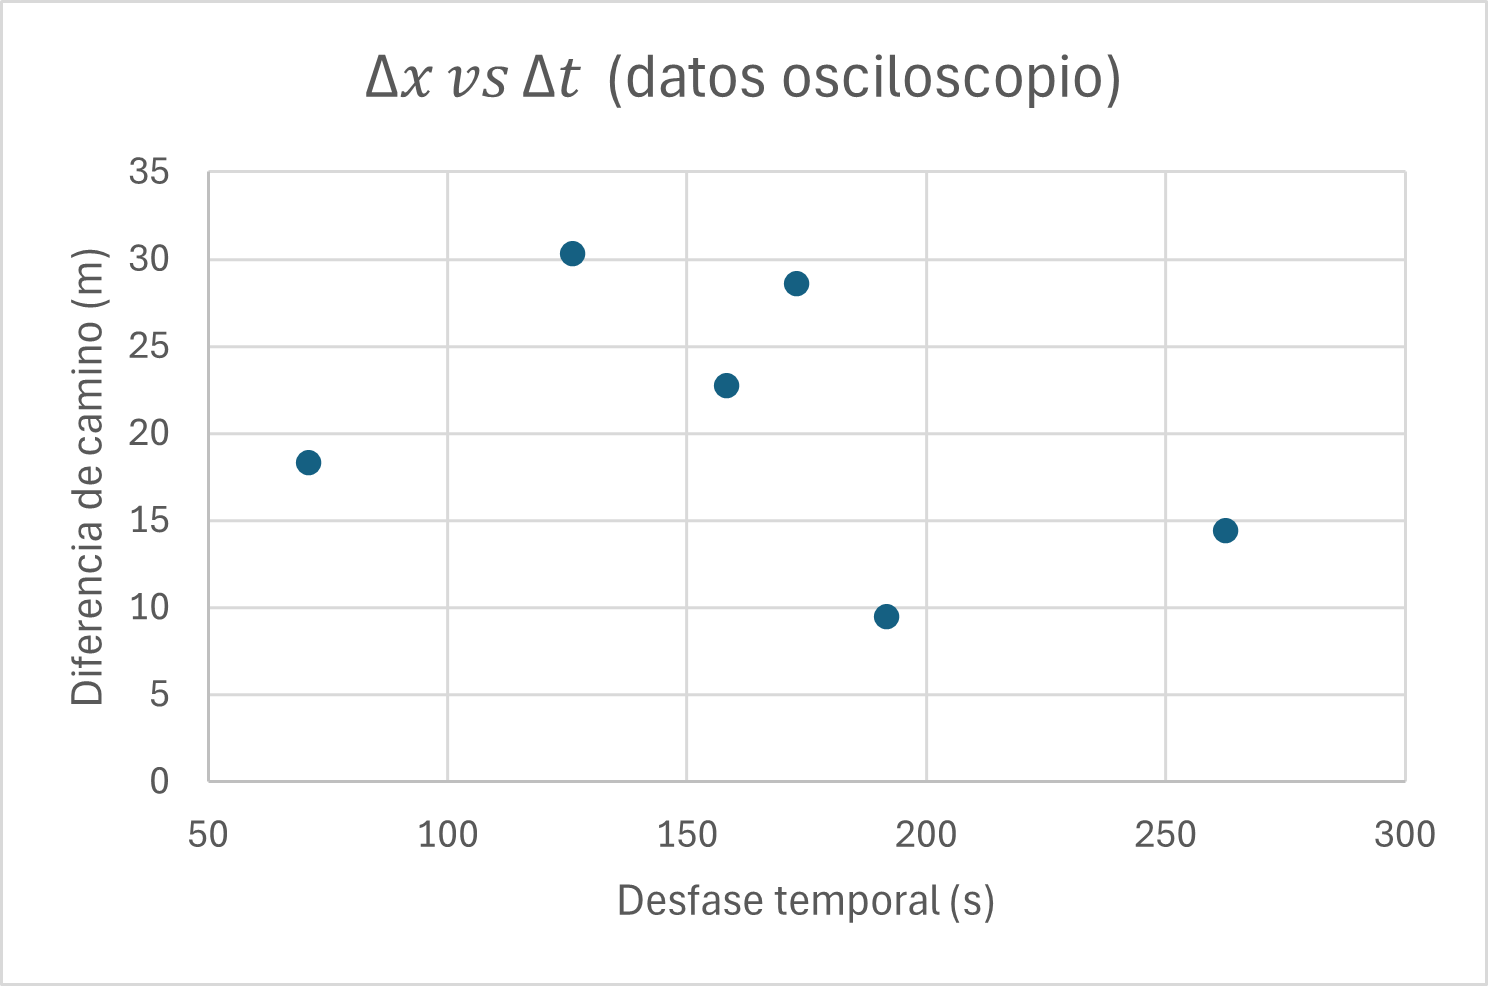
\includegraphics[width=\linewidth]{n-4.2.png} % Ruta de la quinta imagen
        \caption{Medida n4.2}
        \label{fig:n4.2}
    \end{subfigure}

    \caption{Gráfica de los puntos encontrados para cada medida realizada.}
    \label{fig:C_resultados_malos}
\end{figure}

 La medida n1 fué la más cercana al valor esperado de $c$, sin embargo igual cuenta con una gran incertidumbre. Las medidas n2 y n3 tienen pendientes con un orden de magnitud menor al esperado, y en el caso de la n3 la pendiente tiene signo negativo, lo cual carece de sentido. Así mismo carece de sentido los resultado de la medida n4, para la cual se incluyen aquí los resultados obtenidos tanto por la pantalla del osciloscopio como por el tratamiento de los datos digitales, en este último caso los puntos no siguen una tendencia lineal por lo cual no se pueden analizar.
 
En vista de la falta de precisión encontrada con este experimento, se realizaron algunas mejoras al mismo que se detallan en la siguiente sección.

\subsection{Mejoras del método experimental}

\begin{itemize}
    \item Se encontró que mover la lente convergente mínimamente ocasiona un gran desfase en la señal, por lo que se cambió la lente por una con una distancia focal pequeña y se fabricó un soporte fijo para la misma.
    \item Todos los elementos del montaje se colocaron cuidadosamente a la misma altura, esto con el fin de evitar que el haz de luz incidiera en la lente en diferentes ángulos según se acercara el espejo. Esta mejora también evita que existan discrepancias entre la medida hecha con la cinta y la diferencia de camino real entre los haces, dada por el angulo adicional que puedan tener los haces respecto a la horizontal.
    \item Tomar más medidas mejora la estadística y por ende la precisión, de modo que se aumento la cantidad de valores registrados, de 7 puntos a 15.
    \item Para lograr la mejora anterior también se cambió el lugar de la realización del experimento, a partir de ahora sería el pasillo, el cual es más amplio, permitiendo abarcar distancias mucho más grandes para el recorrido del haz.
\end{itemize}

Posterior a las mejoras mencionadas, se realizó la medida 5, cuyas rectas se incluyen en la figura \ref{fig:C_resultados_no_tan_malos} para los datos tomados en pantalla, n5.1, y los obtenidos por el archivo csv, n5.2.  En este caso se nota la mejoría a simple vista, ya que la recta es evidente; los valores de las pendientes se encuentran en la tabla \ref{tab:C_resultados_no_tan_malos}. Para la recta n5.1 el valor encontrado de la velocidad de la luz difiere con el valor aceptado por tan solo $1\%$, mientras que la medida n5.2 se aleja en $6\%$; sin embargo, esta última cuenta con una precisión mayor. Conociendo el experimento, los equipos con los que se cuenta y la precisión que se puede llegar con ellos cabe la pregunta ¿qué precisión se debe alcanzar con este método para lograr verificar la hipótesis de Céspedes-Curé en las tres localidades planteadas?.


\begin{table}[h]
\centering
\begin{tabular}{|l|l|c|}
\hline
n &  Pendiente (m/s$^2$) & Error Porcentual\\
\hline
5.1 & $(3.0296\pm 0.0556)\times 10^8$ & $1\%$ \\

5.2 & $(3.1965\pm0.0355)\times10^8$ & $6\%$ \\

\hline
\end{tabular}
\caption{Valores de pendiente junto al error porcentual con respecto al valor aceptado de $c$, para la medida realizada después de las mejoras al método experimental.}
\label{tab:C_resultados_no_tan_malos}
\end{table}

\begin{figure}[h!]
    % Primera fila
    \begin{subfigure}[b]{0.5\linewidth}
        \centering
        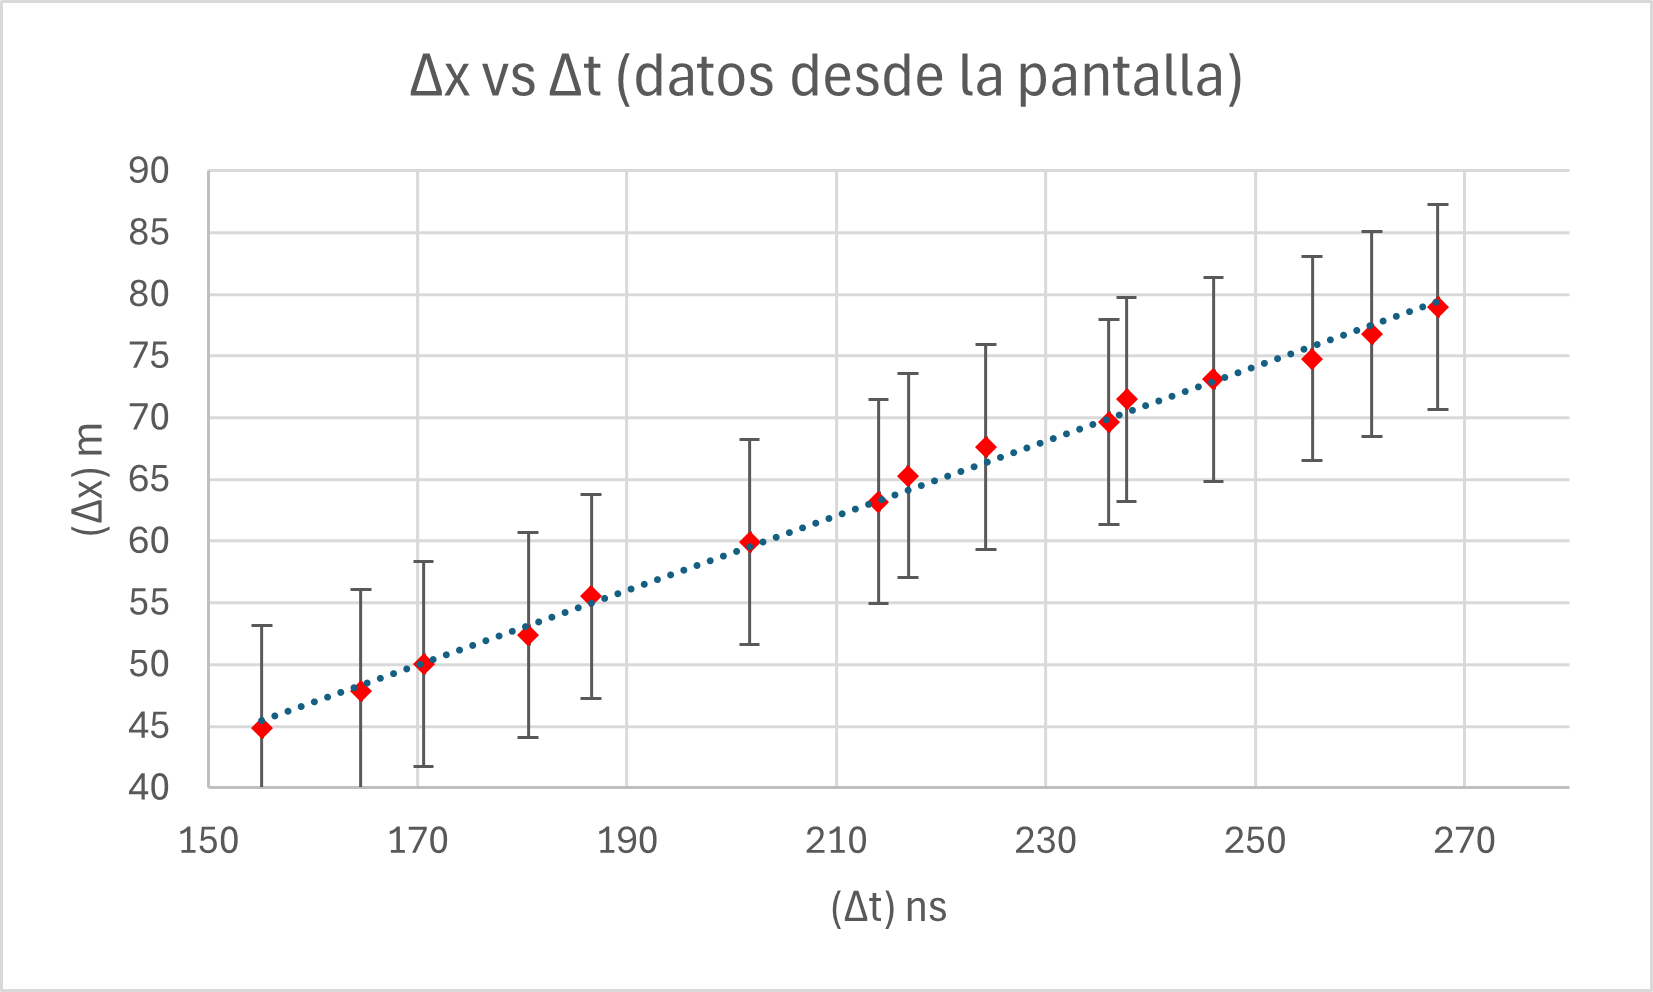
\includegraphics[width=\linewidth]{n-5.1.png} 
        \caption{Medida n5.1}
        \label{fig:n5.1}
    \end{subfigure}
    \hfill
    \begin{subfigure}[b]{0.5\linewidth}
        \centering
        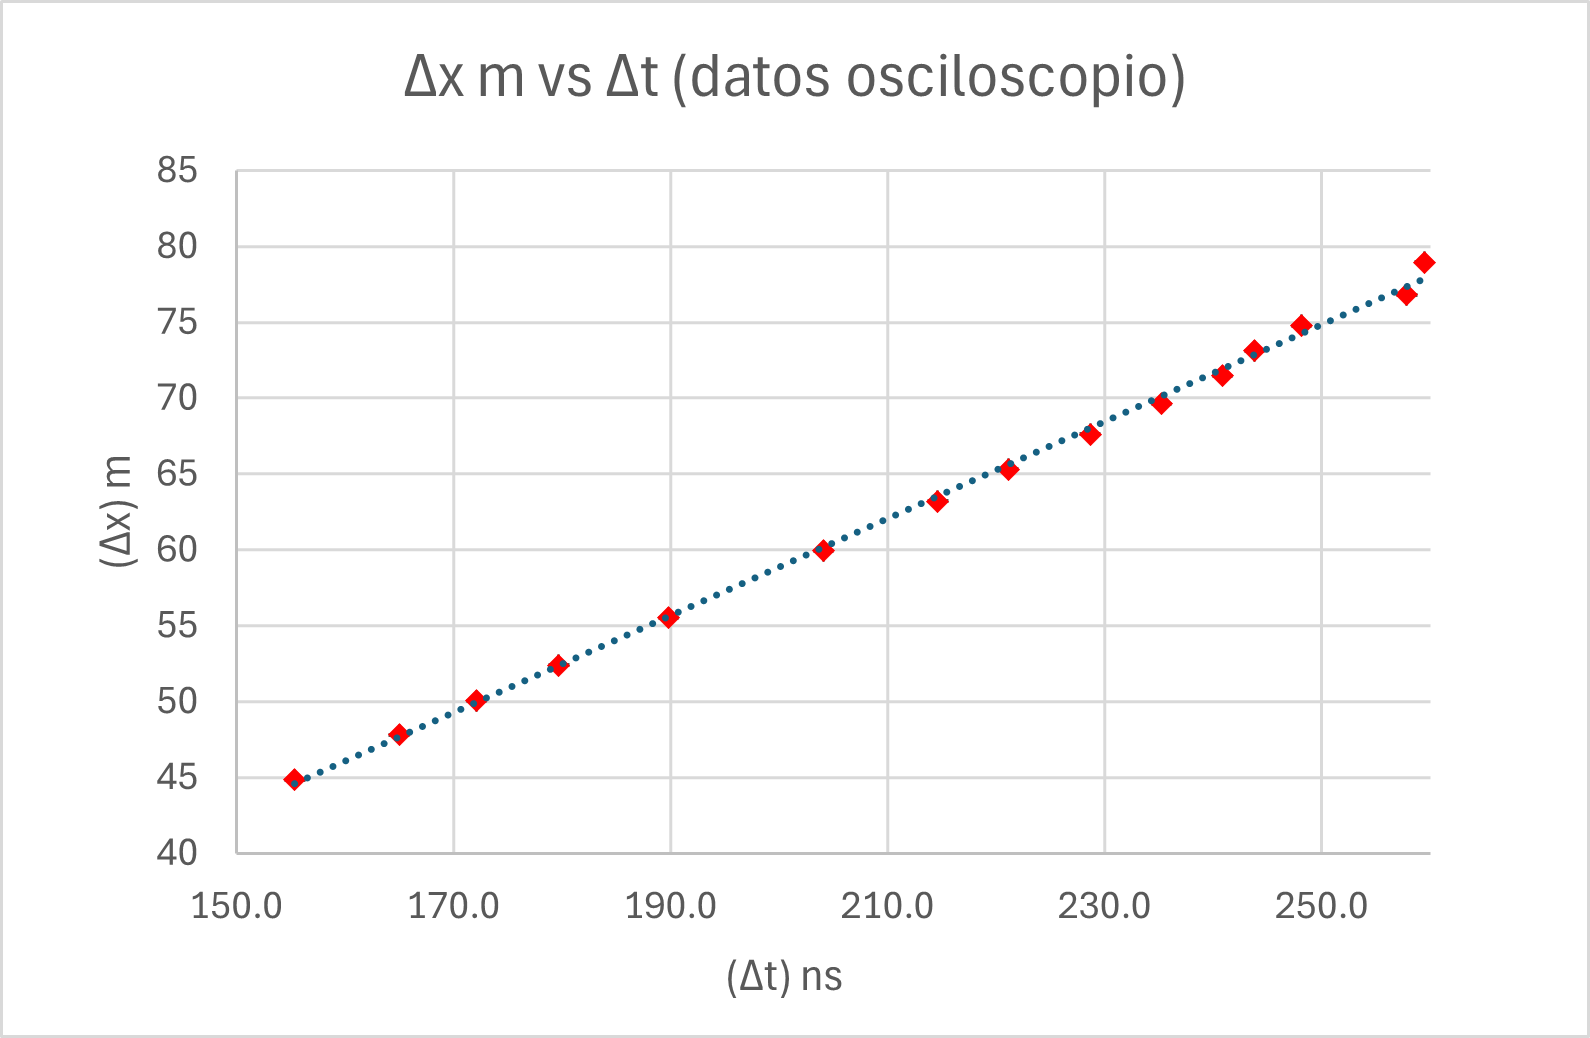
\includegraphics[width=\linewidth]{n-5.2.png} % Ruta de la segunda imagen
        \caption{Medida n5.2}
        \label{fig:n5.2}
    \end{subfigure}
        \caption{Gráfica de los puntos encontrados la mediada realizada despues de aplicar las mejoras, en ambas gráficas se incluyen las barras de error.}
    \label{fig:C_resultados_no_tan_malos}
\end{figure}


\section{Cálculo de la precisión necesaria}


A partir de las velocidades de la luz predichas por la \ac{HCC} para cada localidad, incluidas en la tabla \ref{tab:Valores_c_esperados}, se concluye que el error en las medidas debe ser como máximo de 1 m/s para poder realmente distinguir entre los valores de c y verificar (o no) el cumplimiento de la hipótesis. En este primer experimento para calcular c se usa la siguiente ecuación  
\begin{equation}
    c = \frac{\Delta x}{\Delta t}
\end{equation}
que es la diferencia de camino entre diferencia de tiempo (desfase) entre cada haz de luz que provienen originalmente del mismo láser.  La propagación de errores de dicha ecuación es simplemente

\begin{equation}
    E_c = \frac{E_{\Delta x}}{\Delta t} + \frac{\Delta x}{(\Delta t)^2} E_{\Delta t} 
\end{equation}

Sea $\kappa$ una fracción de la unidad, $0 < \kappa < 1$ , y $F$ otra tal que $F = 1 – \kappa$ entonces podemos dividir el error anterior en sus dos componentes, por una parte

\begin{equation}
    \kappa \cdot E_c = \frac{E_{\Delta x}}{\Delta t} \implies E_{\Delta x} = \kappa \cdot E_c \cdot \Delta t
\end{equation}

y por otra parte

\begin{equation}
    F \cdot E_c = \frac{\Delta x}{(\Delta t)^2} E_{\Delta t} \implies E_{\Delta t} = F \cdot E_c \cdot \frac{(\Delta t)^2}{\Delta x}
\end{equation}

Para estimar los valores de los errores de distancia y tiempo consideremos un error de $c$ de  $E_c = 1$m/s. Para  $\Delta t$ los valores obtenidos están en el orden de los cientos de nano segundos, digamos 200 ns  es decir    $\Delta t= 2 \times 10^{-7}$s y las diferencias de distancias, cuando se hicieron mediciones en el pasillo, estuvieron entre $40$m y $80$m , así que tomemos   $\Delta x= 60$ m como valor representativo. Finalmente, usando los valores detallados anteriormente se tiene que
\begin{align}
    E_{\Delta x} &\sim \kappa \cdot 2 \times 10^{-7} \text{ m} \\
    E_{\Delta t} &\sim F \cdot 6.67 \times 10^{-16} \text{ s}
\end{align}

Entonces, para obtener una velocidad de la luz con una precisión aceptable para diferenciar el efecto de la \ac{HCC} usando este método experimental es necesario que las diferencias de camino sean medidas con una precisión de decenas de nanómetros y las medidas de desfase con precisión de algunos femtosegundos. Es evidente que estas precisiones se escapan de nuestra capacidad. Para la distancia se usa una cinta métrica cuya apreciación es de un milímetro, alcanzar precisiones de nanómetros cuando se miden distancias tan grandes como $80$ m es una tarea complicada. Así mismo ocurre en el caso de la precisión en la medida de desfase, incluso con el osciloscopio y el cálculo de mejor ajuste con Python los errores para los $\Delta t$   están alrededor de $2 \times 10 ^{-10}$ s.

Con el fin de dimensionar y contextualizar la magnitud de la precisión de $c$ que se necesita, consideremos la medición de la velocidad de la luz realizada por Evenson y colaboradores en 1972 \cite{Evenson1972Speed}. En dicho experimento se encontró un valor de c de 299792456.2(1.1) m/s, es decir, una apreciación de la medida parecida a la necesaria para verificar la hipótesis de Cespedes-Curé. El valor encontrado en 1972 es uno de los más precisos y contribuyó a la adopción de la constante de la velocidad de la luz en el vacío como valor definitorio del metro como unidad de distancia. El experimento de Evenson consistía en una medida directa de $c$ pero usando la relación $c=f \lambda$ donde se midió directamente la frecuencia $f$ y la longitud de onda $\lambda$ de la radiación de un láser estabilizado. Para lograr la estabilización del láser y la correcta medición se requieren equipos a los que actualmente no tenemos acceso; por lo tanto, se planteó un nuevo experimento que busca realizar una medición indirecta del efecto de la densidad de energía gravitacional sobre la velocidad de la luz.
